% Charlotte Geiger - Manuel Lippert - Leonard Schatt
% Physikalisches Praktikum

% 2.Kapitel Fragen zur Vorbereitung

\chapter{Fragen zur Vorbereitung}
\label{chap:fvz}

% 1
\section{Operationsverstärker und Gegenkopplung}
\label{sec:dataOPV}
Bei einem realen und idealen Operationsverstärker (OPV) sind folgende Größen wichtig:
\begin{itemize}
    \item Verstärkung $V$ (möglichst groß)
    \item Eingangswiderstand $R_e$ (möglichst hoch $\rightarrow$ geringe Belastung für Signalquelle)
    \item Ausgangswiderstand $R_a$ (möglichst klein $\rightarrow$ Ausgangsspannung $U_a$ unabhängig vom Verbraucher)
    \item Bandbreite (Obere Grenzfrequenz) $B=f_{gr}$ (Kleine Einstellzeit $\rightarrow$ hohe Grenzfrequenz $f_{gr}$)
\end{itemize}
\begin{center}
    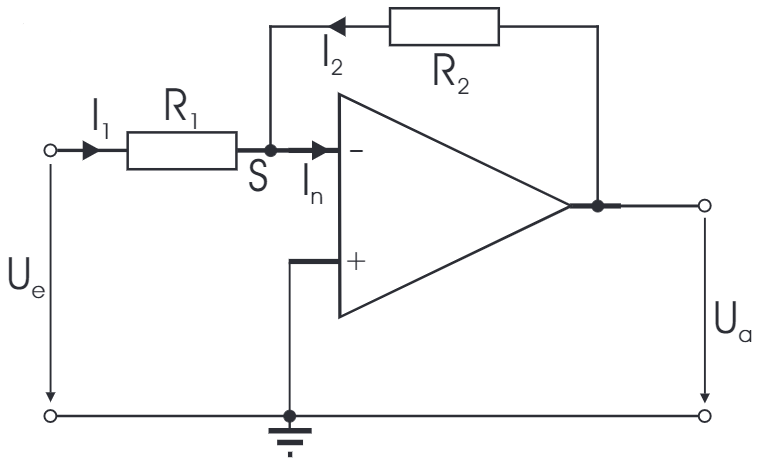
\includegraphics[scale = 0.4]{Gegenkopplung.PNG}
    \captionof{figure}{Gegenkopplung eines invertierenden Verstärkers}
\end{center}
Durch die Gegenkopplung wird unabhängig von Signal- und Ausgangsspannungen immer genau auf dem Potential des nichtinvertierenden Eingangs gehalte, wodurch Ein- und Ausgang voneinander getrennt sind und der Verstärker nicht übersteuern kann. Dabei beeinflusst die Gegenkopplung die Frequenz so, dass die Bandbreite ansteigt, aber die Verstärkung gleichzeitig abnimmt.\\
Das \textbf{Verstärkung–Bandbreite–Produkt} bleibt dabei näherungsweise konstant $v\cdot B = v \cdot f_{gr} = \text{constant}$. Der konstante Bereich wird dabei durch die Grenzfrequenz $f_{gr}$ begrenzt, wobei bei einer Verstärkung $v=0$ die sogenannte \textbf{Transitfrequenz} $f_T$ liegt. %EKS Kapitel 31
\newpage

% 2
\section{Begriffsklärung}
\label{sec:begriffe}
\begin{itemize}
    \item \textbf{Eingangs-Offsetstrom} (Input Offset Current):\\ Eingangsstromdifferenz bei der die Ausgangsspannung des Operationsverstärkers 0 V beträgt. %HBG
    \item \textbf{Eingangs-Offsetspannung} (Input Offset Voltage):\\ Eingangsspannung bei der die Ausgangsspannung des Operationsverstärkers 0 V beträgt. %HBG
    \item \textbf{Gleichtakt-Eingangswiderstand}:\\ Diese beiden Widerstände liegen zwischen dem jeweiligen Eingang und Masseund liegen somit parallel zu den Eingängen und werden durch die Gegenkopplung nicht beeinflusst. Am nichtinvertierenden Eingang bewirkt der Gleichtakt-Eingangswiderstand eine Abschwächung und am invertierenden Eingang eine Steigerung der Verstärkung (Bei realen OPV Abweichungen vernachlässigbar für $<10$ M$\Omega$). %Wikipedia
    \item \textbf{Differenz-Eingangswiderstand}:\\ Dieser Widerstand liegt zwischen nichtinvertierendem und invertierendem Eingang und wirkt durch die Gegenkopplung dynamisch stark erhöhend. Dabei wird die Spannung zwischen den beiden Eingängen nahe 0 V gehalten (Dynamische Werte in Bereich $<10$ G$\Omega$ aufwärts). %Wikipedia
    \item \textbf{Gleichtakt-Eingangsbereich} (Input Common Mode Range):\\ Eingangsspannungsbereich bzgl. der Betriebsspannung, bei dem der OPV linear arbeitet. Wird der Bereich verlassen bricht die Verstärkung drastisch ein und kann Schäden am Bauteil verursachen. 
    \item \textbf{Differenz-Eingangsbereich}:\\ Zulässige Eingangsspannungsdifferenzen, bei dem der OPV normal arbeitet.
    \item \textbf{Slewrate}:\\ Bauartbedingte schnellste Änderung der Ausgangsspannung. Der Wert liegt beim kompensierten OPV fest und kann beim unkompensierten durch externe Beschaltung reduziert werden. %HBS
    \item \textbf{Impedanzwandlung}:\\ Die Verschaltung, bei der der invertierte Eingang mit dem Ausgang kurzgeschlossen/rückgekoppelt ist, um eine gleichphasige Spannung ($U_e=U_a$) und eine Verstärkung $v=1$ zu realisieren. Es gelten Bedingung für $R_e, R_a$ wie in Kapitel 2.1. Damit wird das Signal von einer hochohmigen zu einer niederohmigen Last gewandelt. 
\end{itemize}

% 3
\section{Nichtinvertierender Verstärker}
\label{sec:noninvertedOPV}
\begin{center}
    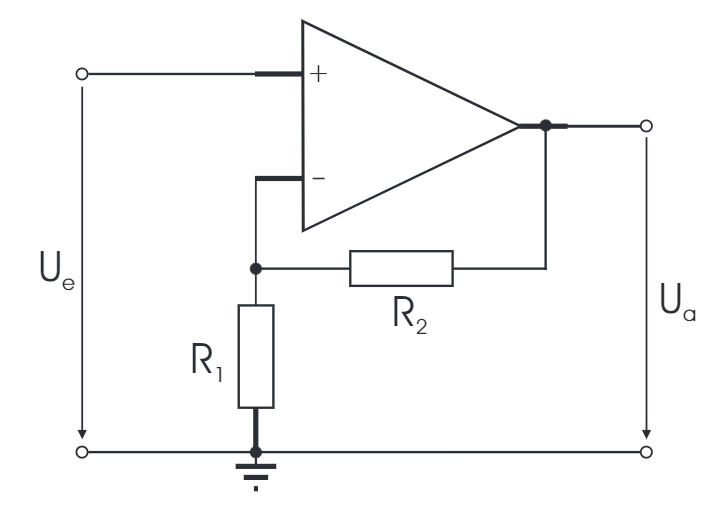
\includegraphics[scale = 0.4]{noninvertedOPV.PNG} %Pfeile
    \captionof{figure}{Nichtinvertierender Verstärker}
\end{center}
Aus den Annahmen aus dem Skript (EL2 - 2) folgt:
\begin{gather}
    U_n - U_p = \Delta U = 0\\
    \Rightarrow
    \begin{aligned}
        U_e&= \Delta U + U_{R_1} = U_{R_1}\\
        U_a&= U_{R_1} + U_{R_2}
    \end{aligned}\\[0.5cm]
    I_n = I_p = 0\\
    \Rightarrow I_1 + I_n = I_1 = I_2 =: I~\text{(Aus Knotenregel)}
\end{gather}
Womit sich die Verstärkung angeben lässt wie folgt:
\begin{gather}
    v = \frac{U_a}{U_e} = \frac{U_{R_1} + U_{R_2}}{U_{R_1}} = \frac{I (R_1+R_2)}{I R_1} = 1 + \frac{R_2}{R_1}\\[0.5cm]
    \Rightarrow \boxed{v = 1 + \frac{R_2}{R_1}}
\end{gather}

% 4
\section{Integrationsschaltung}
\label{sec:intschaltung}
\begin{center}
    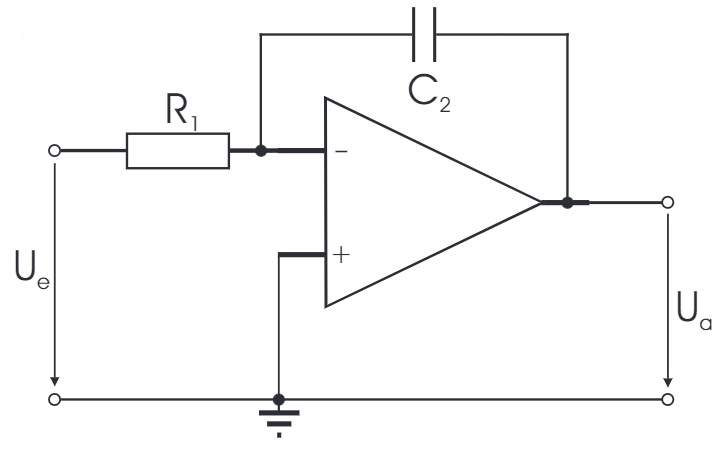
\includegraphics[scale = 0.4]{intOPV.PNG} %Pfeile
    \captionof{figure}{Integrationsschaltung}
\end{center}
Mit den selben Annahmen aus Kapitel 2.3 folgt:
\begin{gather}
    I_1 + I_{C_2} = 0\\
    I_1 = \frac{U_e}{R_1}
\end{gather}
Weiterhin ist die zeitliche Ladungsänderung am Kondensator $C_2$ gegeben durch die zeitliche Änderung der Ausgangsspannung und kann ausgedrückt werden als
\begin{gather}
    \dot{Q_{C_2}} = C_2 \dot{U_a} = I_{C_2}~.
\end{gather}
Mit Gleichung (2.7) und (2.8) folgt:
\begin{gather}
    \begin{aligned}
        \frac{U_e}{R_1} &= -C_2 \dot{U_a}\\
        \Leftrightarrow \dot{U_a} &= -\frac{1}{R_1 C_2} U_e\\[0.5cm]
        %\text{Homogene Differentialgleichung 1.Ordnung}
    \end{aligned}
\end{gather}
Die Gleichung (2.10) ist eine Differentialgleichung 1. Ordnung mit allgemeiner Lösung:
\begin{gather}
    \Rightarrow \boxed{U_a(t) = -\frac{1}{R_1 C_2} \int_0^t U_e(\tau)\text{d}\tau + U_0}
\end{gather}
Dabei ist $U_0$ festgelegt durch die Aufladung des Kondensators und somit gilt $U_0 = U_{C_2}$, wobei fortan zum vereinfachen der Rechnung $U_0=0~\text{V}$ angenommen wird.\\
\begin{gather}
    \text{\textbf{Ansatz:}}~U_e(t) = U_{e,0}e^{i\omega t}\\
    \Rightarrow U_a(t) = -\frac{1}{R_1 C_2} \frac{1}{i\omega} U_{e,0}(e^{i\omega t}-1) \overset{t \gg 0}{\approx} -\frac{1}{R_1 C_2} \frac{1}{i\omega} U_{e,0}e^{i\omega t}\\[0.5cm]
    \Rightarrow v_{1}(\omega) = \abs{\frac{U_a}{U_e}} = \abs{-\frac{1}{R_1 C_2} \frac{1}{i\omega}} = \frac{1}{R_1 C_2 \omega}\\[0.5cm]
    \Rightarrow \boxed{v_{i,1}(\omega)=\frac{1}{R_1 C_2 \omega}}
\end{gather}
Schaltet man nun zum Kondensator $C_2$ noch den Widerstand $R_2$ parallel gilt:
\begin{gather}
    I_1 + I_2 + I_{C_2} = 0\\
    \begin{aligned}
        \Rightarrow \frac{U_e}{R_1} + \frac{U_a}{R_2} &= -C_2 \dot{U_a}\\
        \Leftrightarrow \dot{U_a} + \frac{U_a}{R_1 C_2} &= -\frac{U_e}{R_2 C_2}\\
        %\text{Inhomogene Differentialgleichung 1.Ordnung}
    \end{aligned}
\end{gather}
Bei Gleichung (2.17) handelt es sich um eine Inhomogene lineare Differentialgleichung 1.Ordnung dessen Lösung wie folgt bestimmt wird:
\begin{gather}
    \text{\textbf{Ansatz:}}~U_a^\text{h}(t) = U_{a,0}~e^{-\frac{1}{R_2 C_2} t}\\
    \begin{aligned}
        \Rightarrow U_a(t) &= K(t) U_a^\text{h}(t)~\text{,wobei}~K(t) = -\frac{1}{R_1 C_2} \int_0^t\frac{U_e(\tau)}{U_a^\text{h}(\tau)}\text{d}\tau\\
        \Rightarrow U_a(t) &= -\frac{1}{R_1 C_2} \int_0^t \frac{U_e(\tau)}{U_a^\text{h}(\tau)}\text{d}\tau U_a^\text{h}(t)\\
        &= -\frac{U_{e,0}}{R_1 C_2} \int_0^t e^{\left(i\omega + \frac{1}{R_2 C_2}\right) \tau} \text{d}\tau~e^{-\frac{1}{R_2 C_2} t}\\
        &= -\frac{U_{e,0}}{R_1 C_2} \frac{1}{i\omega + \frac{1}{R_2 C_2}} \left(e^{\left(i\omega + \frac{1}{R_2 C_2}\right) t} - 1 \right) ~e^{-\frac{1}{R_2 C_2} t}\\
        &\overset{t \gg 0}{\approx} -\frac{U_{e,0}}{R_1 C_2} \frac{1}{i\omega + \frac{1}{R_2 C_2}} e^{\left(i\omega + \frac{1}{R_2 C_2}\right) t}~e^{-\frac{1}{R_2 C_2} t}\\
        &= - \frac{R_2}{R_1} \frac{1}{1+i\omega R_2 C_2} U_{e,0} e^{i\omega t} = - \frac{R_2}{R_1} \frac{1}{1+i\omega R_2 C_2} U_e(t)\\[0.5cm]
        \Rightarrow v_{2}(\omega) &= \abs{-\frac{R_2}{R_1} \frac{1}{1+i\omega R_2 C_2}} = \frac{R_2}{R_1} \frac{1}{\sqrt{1+(\omega R_2 C_2)^2}}
    \end{aligned}\\[0.5cm]
    \Rightarrow \boxed{v_{i,2}(\omega)=\frac{R_2}{R_1} \frac{1}{\sqrt{1+(\omega R_2 C_2)^2}}}
\end{gather}
Bei der Grenzfrequenz $f_{gr}$ soll die Verstärkung $v$ ungefähr $70\%~\approx\frac{1}{\sqrt{2}}$ der Leerlaufverstärkung $v(0)$ betragen, wobei diese gemessen wird wenn der OPV nicht beschalten ist. Damit ist $v(0)$ in (EL2 - 3) durch Gleichung (3) gegeben und es folgt: %EKS Kapitel 31 S.264
\begin{gather}
    v_{i,2}(\omega_{i,gr}) = \frac{1}{\sqrt{2}} v(0) = \frac{1}{\sqrt{2}} \frac{R_2}{R_1} \overset{!}{=} \frac{R_2}{R_1} \frac{1}{\sqrt{1+(\omega_{i,gr} R_2 C_2)^2}}\\
    \Leftrightarrow \boxed{w_{i,gr} = \frac{1}{R_2 C_2}}
\end{gather}
Um die Ausdrücke für die Verstärkung zu vereinfachen wenden wir folgende Formeln an:
\begin{gather}
    \omega R_2 C_2 = \frac{\omega}{\omega_{i,gr}} = \tilde{\omega}_i\\
    v\frac{R_1}{R_2}=\tilde{v}\\
    \Rightarrow \boxed{\tilde{v}_{i,1}(\tilde{\omega}_i) = \frac{1}{\tilde{\omega}_i} \tab \tilde{v}_{i,2}(\tilde{\omega}_i) =\frac{1}{\sqrt{1+\tilde{\omega}_i^2}}}
\end{gather}
Dabei ist anzumerken, dass auf die Umwandlung auf die Frequenz $f=2\pi\omega$ verzichtet wird, da die Formeln die selben bleiben.\\
Im folgenden wird $\tilde{v}_1(\tilde{\omega})~\text{und}~\tilde{v}_{2}(\tilde{\omega})$ doppellogarithmisch gegen $\tilde{\omega}$ aufgetragen, womit man Abbildung 2.4 erhält.
\begin{center}
    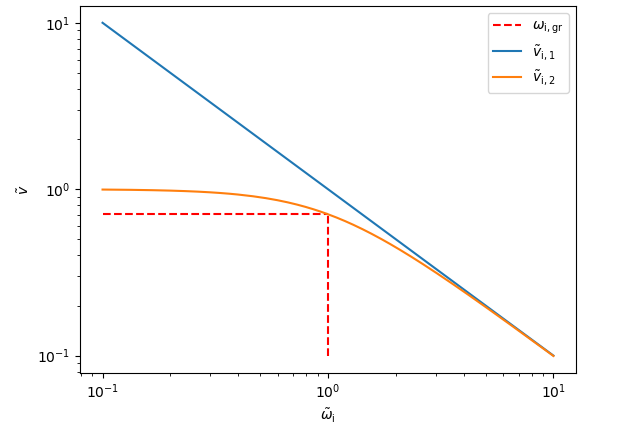
\includegraphics[scale = 0.7]{intOPVlog.png}
    \captionof{figure}{Frequenzabhängigkeit von $\tilde{v}$ zu $\tilde{\omega}_i$}
\end{center}
Aus der Abbildung 2.4 folgt, dass die Frequenz für die Eingangsspannung deutlich höher als $f_{i,gr}=2\pi\omega_{i,gr}$ gewählt werden, damit man sich im linearen Bereich der Verstärkung befindet.

% 5
\section{Differenzierschaltung}
\label{sec:diffschaltung}
\begin{center}
    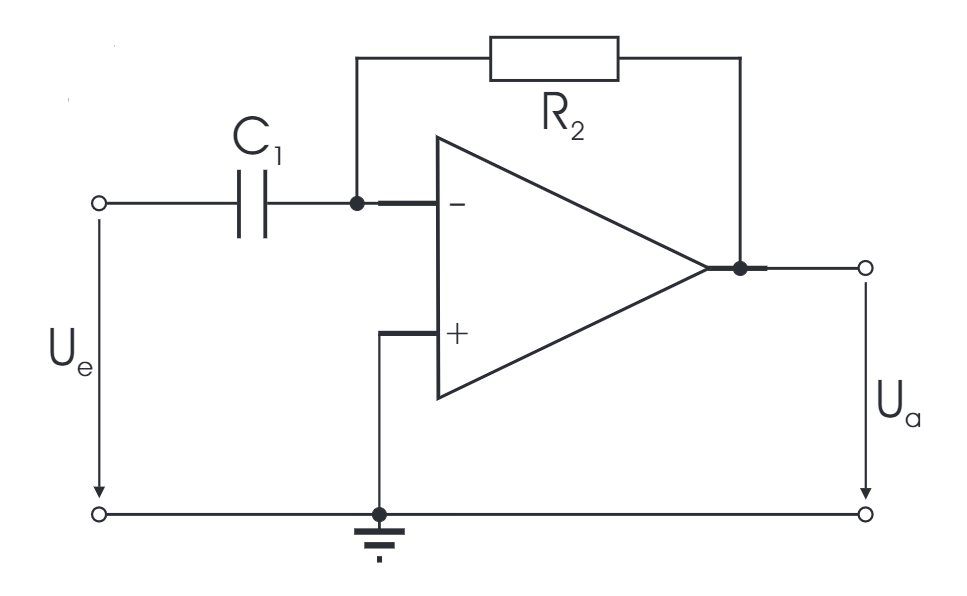
\includegraphics[scale = 0.4]{diffOPV.PNG}
    \captionof{figure}{Differenzierschaltung}
\end{center}
Nochmaliges Anwenden der Annahmen aus Kapitel 2.3 folgt:
\begin{gather}
    I_{C_1} + I_2 = 0\\
    I_2 = \frac{U_a}{R_2}\\
    I_{C_1} = \dot{Q}_{C_1} = C_1 \dot{U_e}
\end{gather}
Einsetzen von (2.26), (2.27) in (2.28) folgt: 
\begin{gather}
    \begin{aligned}
        \Rightarrow \frac{U_a}{R_2}&= -C_1\dot{U_e}\\
        \Leftrightarrow U_a(t)&=-R_2C_1\frac{\text{d}U_e}{\text{d}t}
    \end{aligned}
\end{gather}
Nach Anwendung des selben Ansatzes wie in (2.12) erhält man:
\begin{gather}
    \Rightarrow U_a(t)=-i\omega R_2 C_1 U_e(t)\\[0.5cm]
    \Rightarrow v_1(\omega)=\abs{-i\omega R_2 C_1}=\omega R_2 C_1\\[0.5cm]
    \Rightarrow \boxed{v_{d,1}(\omega) = \omega R_2 C_1}
\end{gather}
Nun wird der Widerstand $R_1$ in Reihe zum Kondensator $C_1$ geschaltet. Betrachtet man Gleichung (2.15), (2.20) und (2.31) wird offensichtlich, dass Verstärkung $v$ der negative Quotient aus Ausgangsimpedanz $Z_{Aus}$ durch Eingangsimpedanz $Z_{Ein}$ ist, woraus folgt: 
\begin{gather}
    v_2(\omega) = \abs{-\frac{Z_{Aus}}{Z_{Ein}}} = \abs{-\frac{R_2}{R_1 + \frac{1}{i\omega C_1}}} = \abs{-\frac{R_2}{R_1} \frac{i\omega R_1C_1}{1+i\omega R_1C_1}} = \frac{R_2}{R_1} \frac{\omega R_1C_1}{\sqrt{1 + (\omega R_1C_1)^2}}\\[0.5cm]
    \Rightarrow \boxed{v_{d,2}(\omega)=\frac{R_2}{R_1} \frac{\omega R_1C_1}{\sqrt{1 + (\omega R_1C_1)^2}}}
\end{gather}
Damit folgt mit dem selben Ansatz wie bei Kapitel 2.4 mit dem unterschied, dass nun statt $v(0)$ nun $v(\Omega\rightarrow \infty)$ betrachtet wird, aber die Gleichung (3) aus (EL2-3) und die Bedingung von für $f_{gr}$ weiterhin gilt:
\begin{gather}
    \boxed{\omega_{d,gr}=\frac{1}{R_1 C_1}}
\end{gather}
Vereinfacht man erneut auf dimensionslose Größen wie in Kapitel 2.4 erhält man:
\begin{gather}
    \boxed{\tilde{v}_{d,1}(\tilde{\omega}_d) = \tilde{\omega}_d \tab \tilde{v}_{d,2}(\tilde{\omega}_d) =\frac{\tilde{\omega}_d}{\sqrt{1+\tilde{\omega}_d^2}}}
\end{gather}
Mit erneuter doppellogarithmischen Auftragung ergibt sich dann Abbildung 2.6 .
\begin{center}
    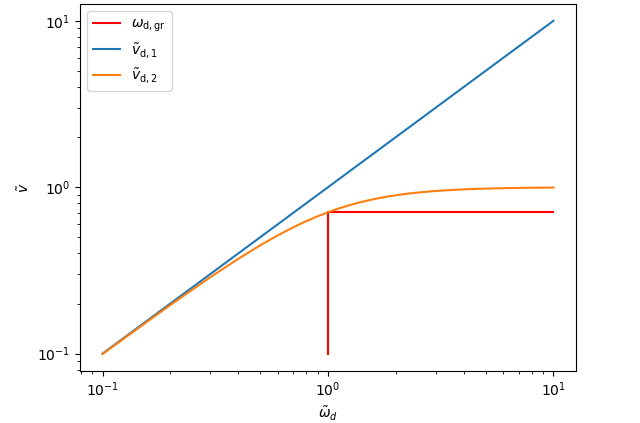
\includegraphics[scale = 0.7]{diffOPVlog.png}
    \captionof{figure}{Frequenzabhängigkeit von $\tilde{v}$ zu $\tilde{\omega}_d$}
\end{center}
An Abbildung 2.6 kann man schon erkennen, dass sie in Prinzip eine spiegelverkehrte Abbildung 2.4 ist. Damit muss aber auch $f_{d,gr}=2\pi\omega_{d,gr}$ kleiner gewählt werden für einen idealen Betrieb des OPV im linearen Bereich.
\newpage
\section*{Bandpass 1.Ordnung}
Diesen Schritt wiederholt man nun nochmal mit, aber nun wird noch zum Widerstand $R_2$ der Kondensator $C_2$ parallel geschaltet, was einer Kombinationsschaltung aus Integration und Differenzierschaltung darstellt. Damit folgt: %http://techniker.pi-pro.de/fs/nae/pdf/filter.pdf
\begin{gather}
    \begin{aligned}
        v_{d,i}(\omega) &= \abs{-\frac{Z_{Aus}}{Z_{Ein}}} = \abs{-\frac{\frac{1}{\frac{1}{R_2}+ i\omega C_2}}{R_1 + \frac{1}{i\omega C_1}}} = \abs{\frac{R_2}{R_1}~\frac{1}{1+i\omega R_2C_2}~\frac{i\omega R_1 C_1}{1+i\omega R_1C_1}}\\
        &=\abs{\frac{R_2}{R_1}\frac{i\omega R_1C_1}{1 + i\omega R_1C_1 + i\omega R_2C_2 + (i\omega R_1C_1)(i\omega R_2C_2)}}\\
        &=\abs{\frac{R_2}{R_1}\frac{1}{1 + \frac{R_2C_2}{R_1C_1} + i\omega R_2C_2 + \frac{1}{i\omega R_1C_1}}}\\
        &=\abs{\frac{1}{\frac{R_1}{R_2}+\frac{C_2}{C_1}+i(\omega R_1C_2 - \frac{1}{\omega R_2C_1})}}
    \end{aligned}\\[0.5cm]
    \Rightarrow \boxed{v_{d,i}=\frac{1}{\sqrt{\left(\frac{R_1}{R_2}+\frac{C_2}{C_1}\right)^2+\left(\omega R_1C_2 - \frac{1}{\omega R_2C_1}\right)^2}}}~\text{mit}~\boxed{\omega_0 = \sqrt{\omega_{i,gr}\cdot \omega_{d,gr}}}
\end{gather}
Mit $R_1 = 2~\Omega, R_2 = \frac{1}{2}~\Omega, C_1 = 2~\text{F}$ und $C_2 = \frac{1}{2}~\text{F}$ erhält man dann Abbildung 2.7 .
\begin{center}
    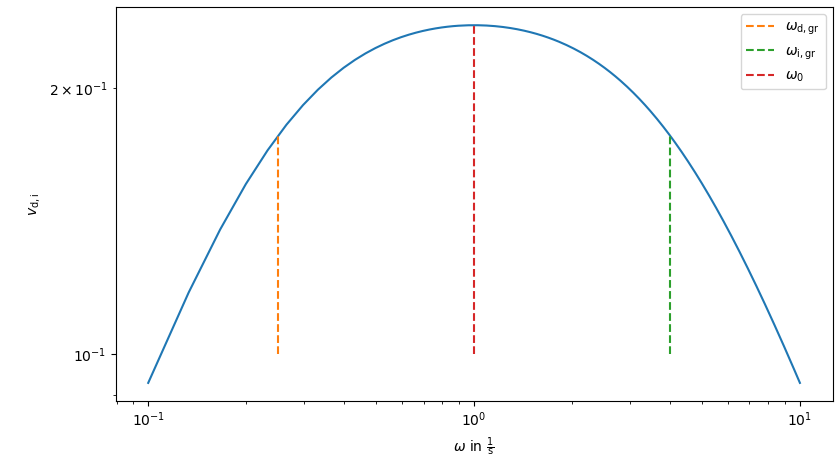
\includegraphics[scale = 0.55]{bandfilter.png}
    \captionof{figure}{Frequenzabhängigkeit von $v$ zu $\omega$}
\end{center}
Die Bandpass wirkt als Differenzierer für $\omega \ll \omega_{d,gr}$ und bei $\omega \gg \omega_{i,gr}$ als Integrierer. Bei geeigneter Wahl von $R_1, R_2, C_1$ und $C_2$ kann der Bandbereich ($\omega \in [\omega_{d,gr},\omega_{i,gr}])$ geschmälert oder verbreitet werden. %HBS